\documentclass[12pt]{article}
\usepackage{hyperref}
\usepackage{fullpage}
\usepackage{anysize} \marginsize{1in}{1in}{1in}{2in}
\usepackage{graphicx}

\begin{document}

\begin{flushright}
	\Huge{\textbf{CS481 Data Science}} \\
	\Large{Assignment 4} \\
	\emph{\large{\today}} \\
	\centering \rule{450pt}{1pt}
	\begin{table}[h!]
		\begin{center}
			\begin{tabular}{lr}
				\large{\textbf{Bilal Khan}} & \large{16K3778}
			\end{tabular}
		\end{center}
	\end{table}
\end{flushright}

\section{K-Means Clustering Using Euclidean Distance}

Using kmeans algorithm and Euclidean distance to cluster the following 8 points into 3 clusters. Using A1 = (2,10), A2 = (2,5), A3 = (8,4), A4 = (5,8), A5 = (7,5), A6 = (6,4), A7 = (1,2) , A8 = (4,9). Consider initial seeds as A1, A4, and A7. Run algorithm for 1 iteration only. At the end of iteration 1, show:
\begin{itemize}
	\item The new clusters (i.e. the examples belong to each cluster)
	\item The centre of the new clusters
	\item Draw 10 x 10 space and all 8 points and show the clusters after 1st iteration and the new centroids
	\item Without running algorithm again, guess how many more iterations are required to converge. Draw the result of each iteration.
\end{itemize}

\begin{figure}
  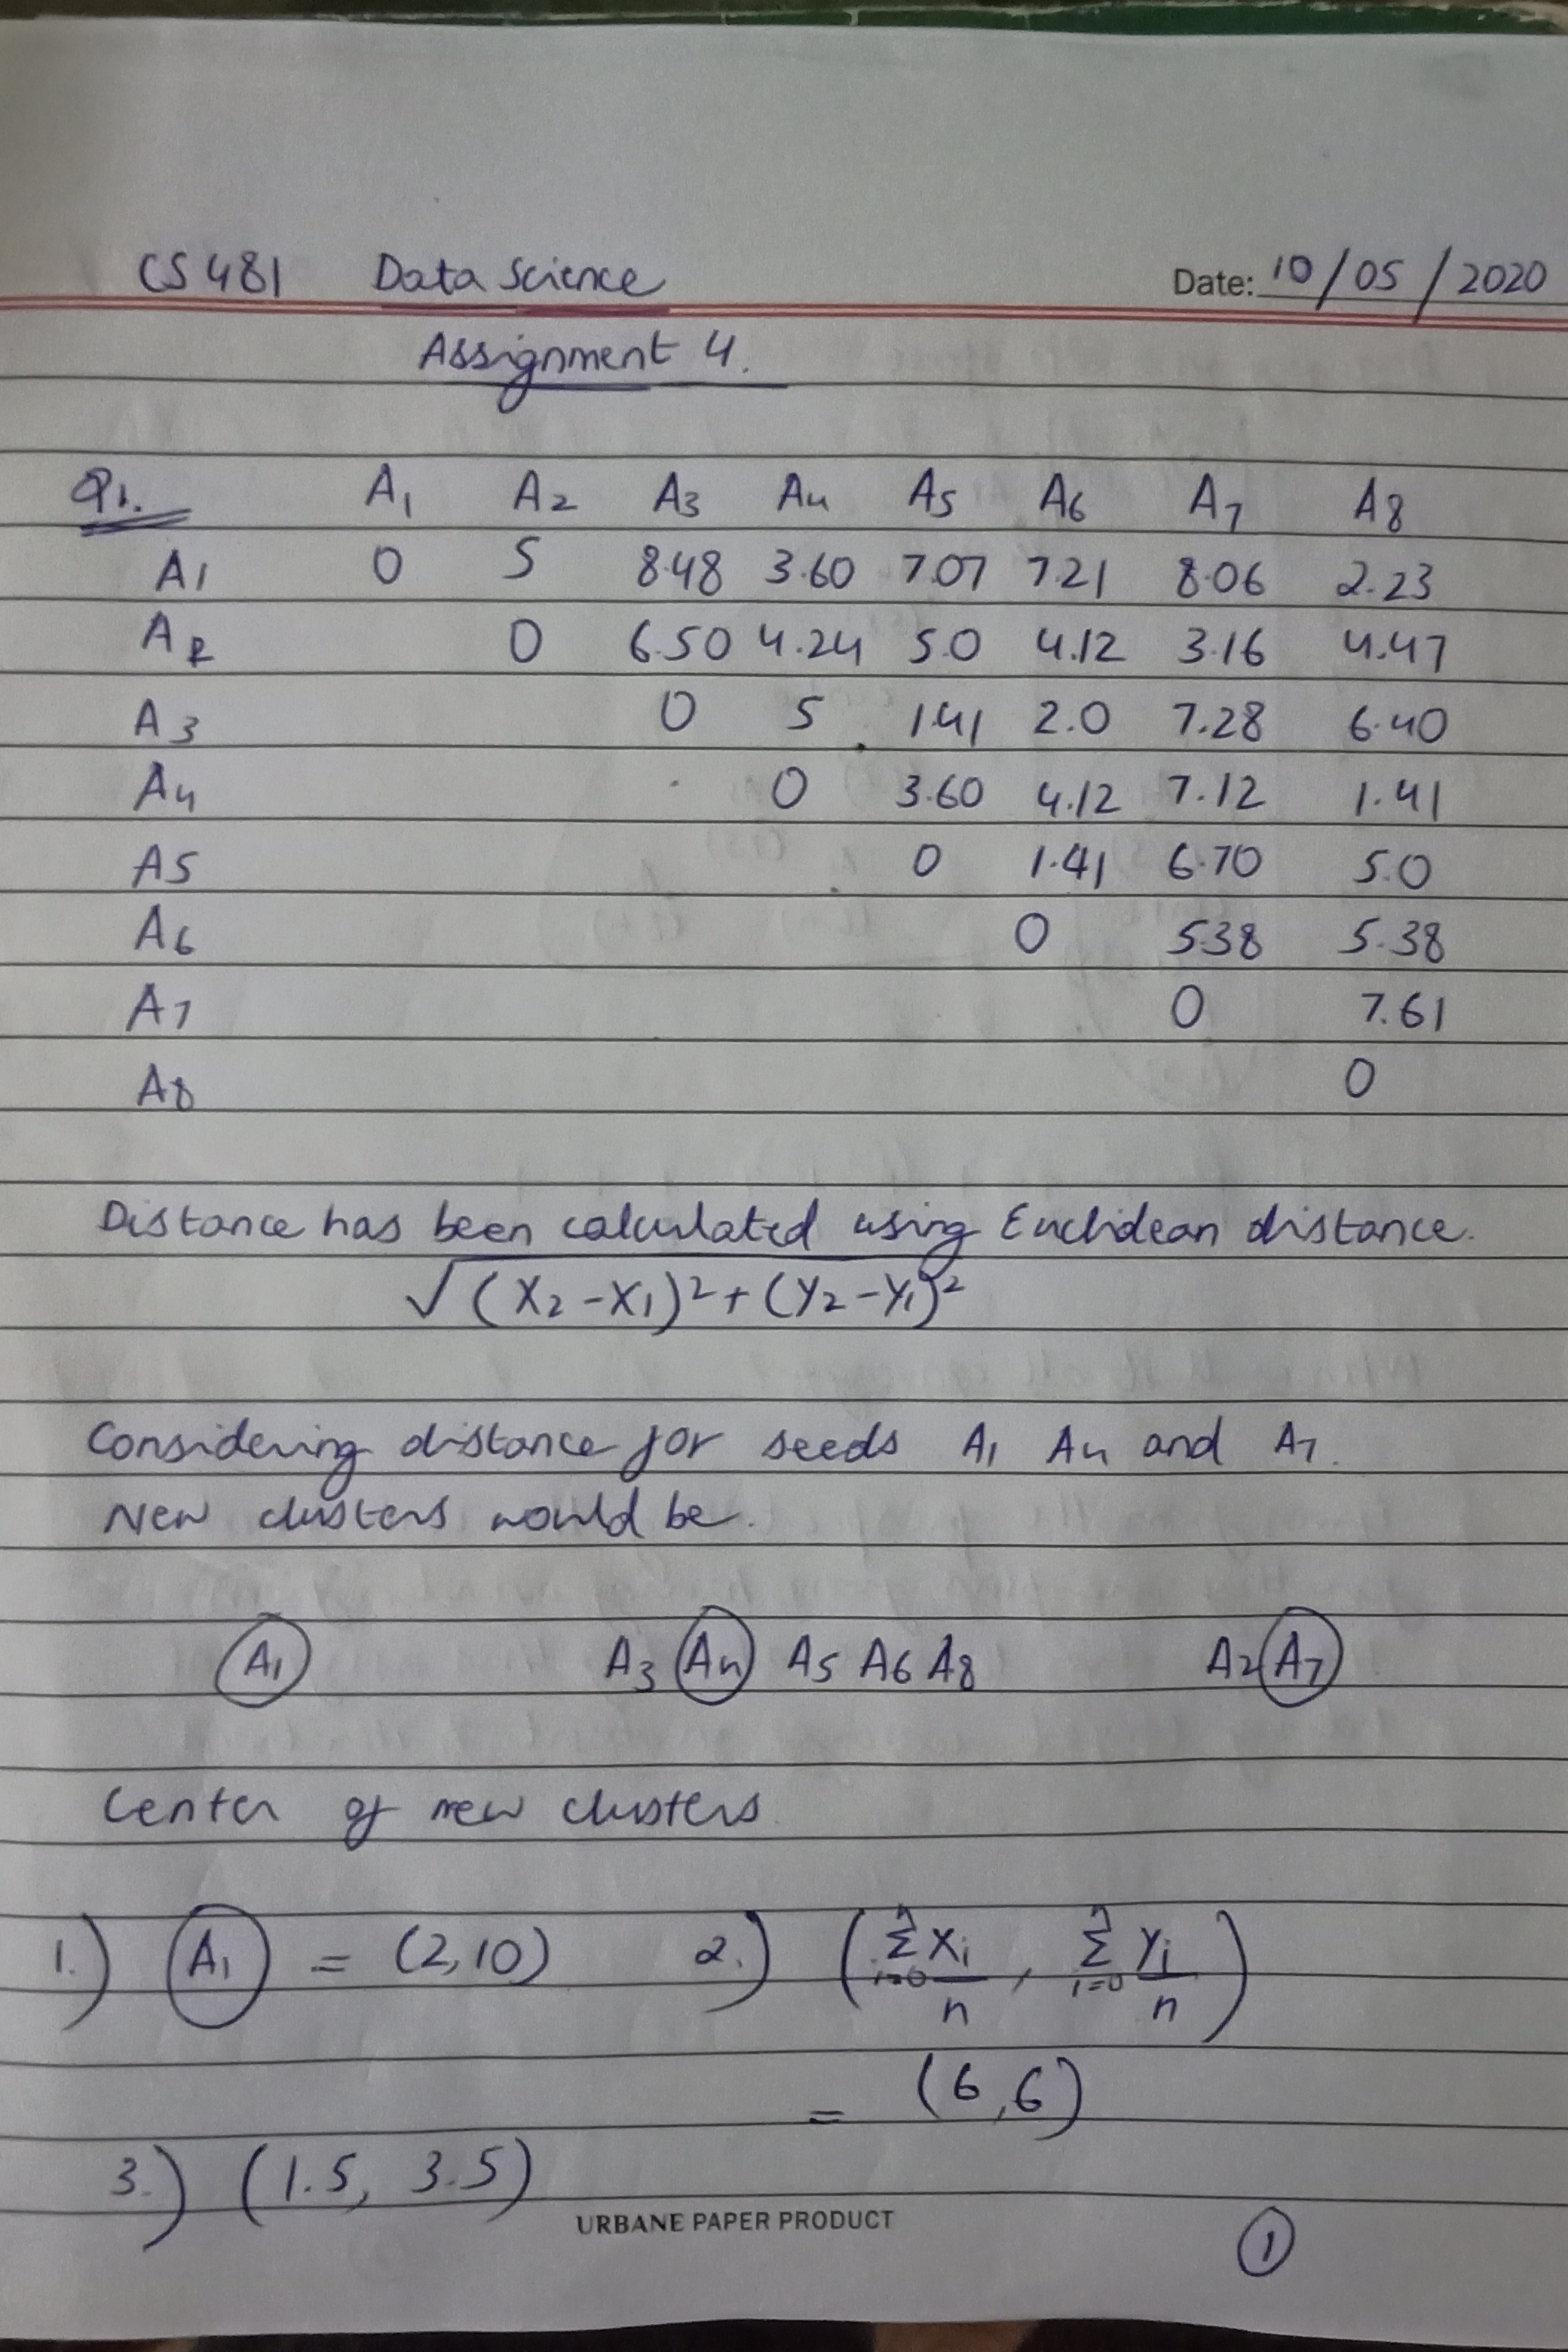
\includegraphics[width=\linewidth]{1.jpg}
  \caption{Clustering iteration and centroid}
  \label{pic1}
\end{figure}

\begin{figure}
  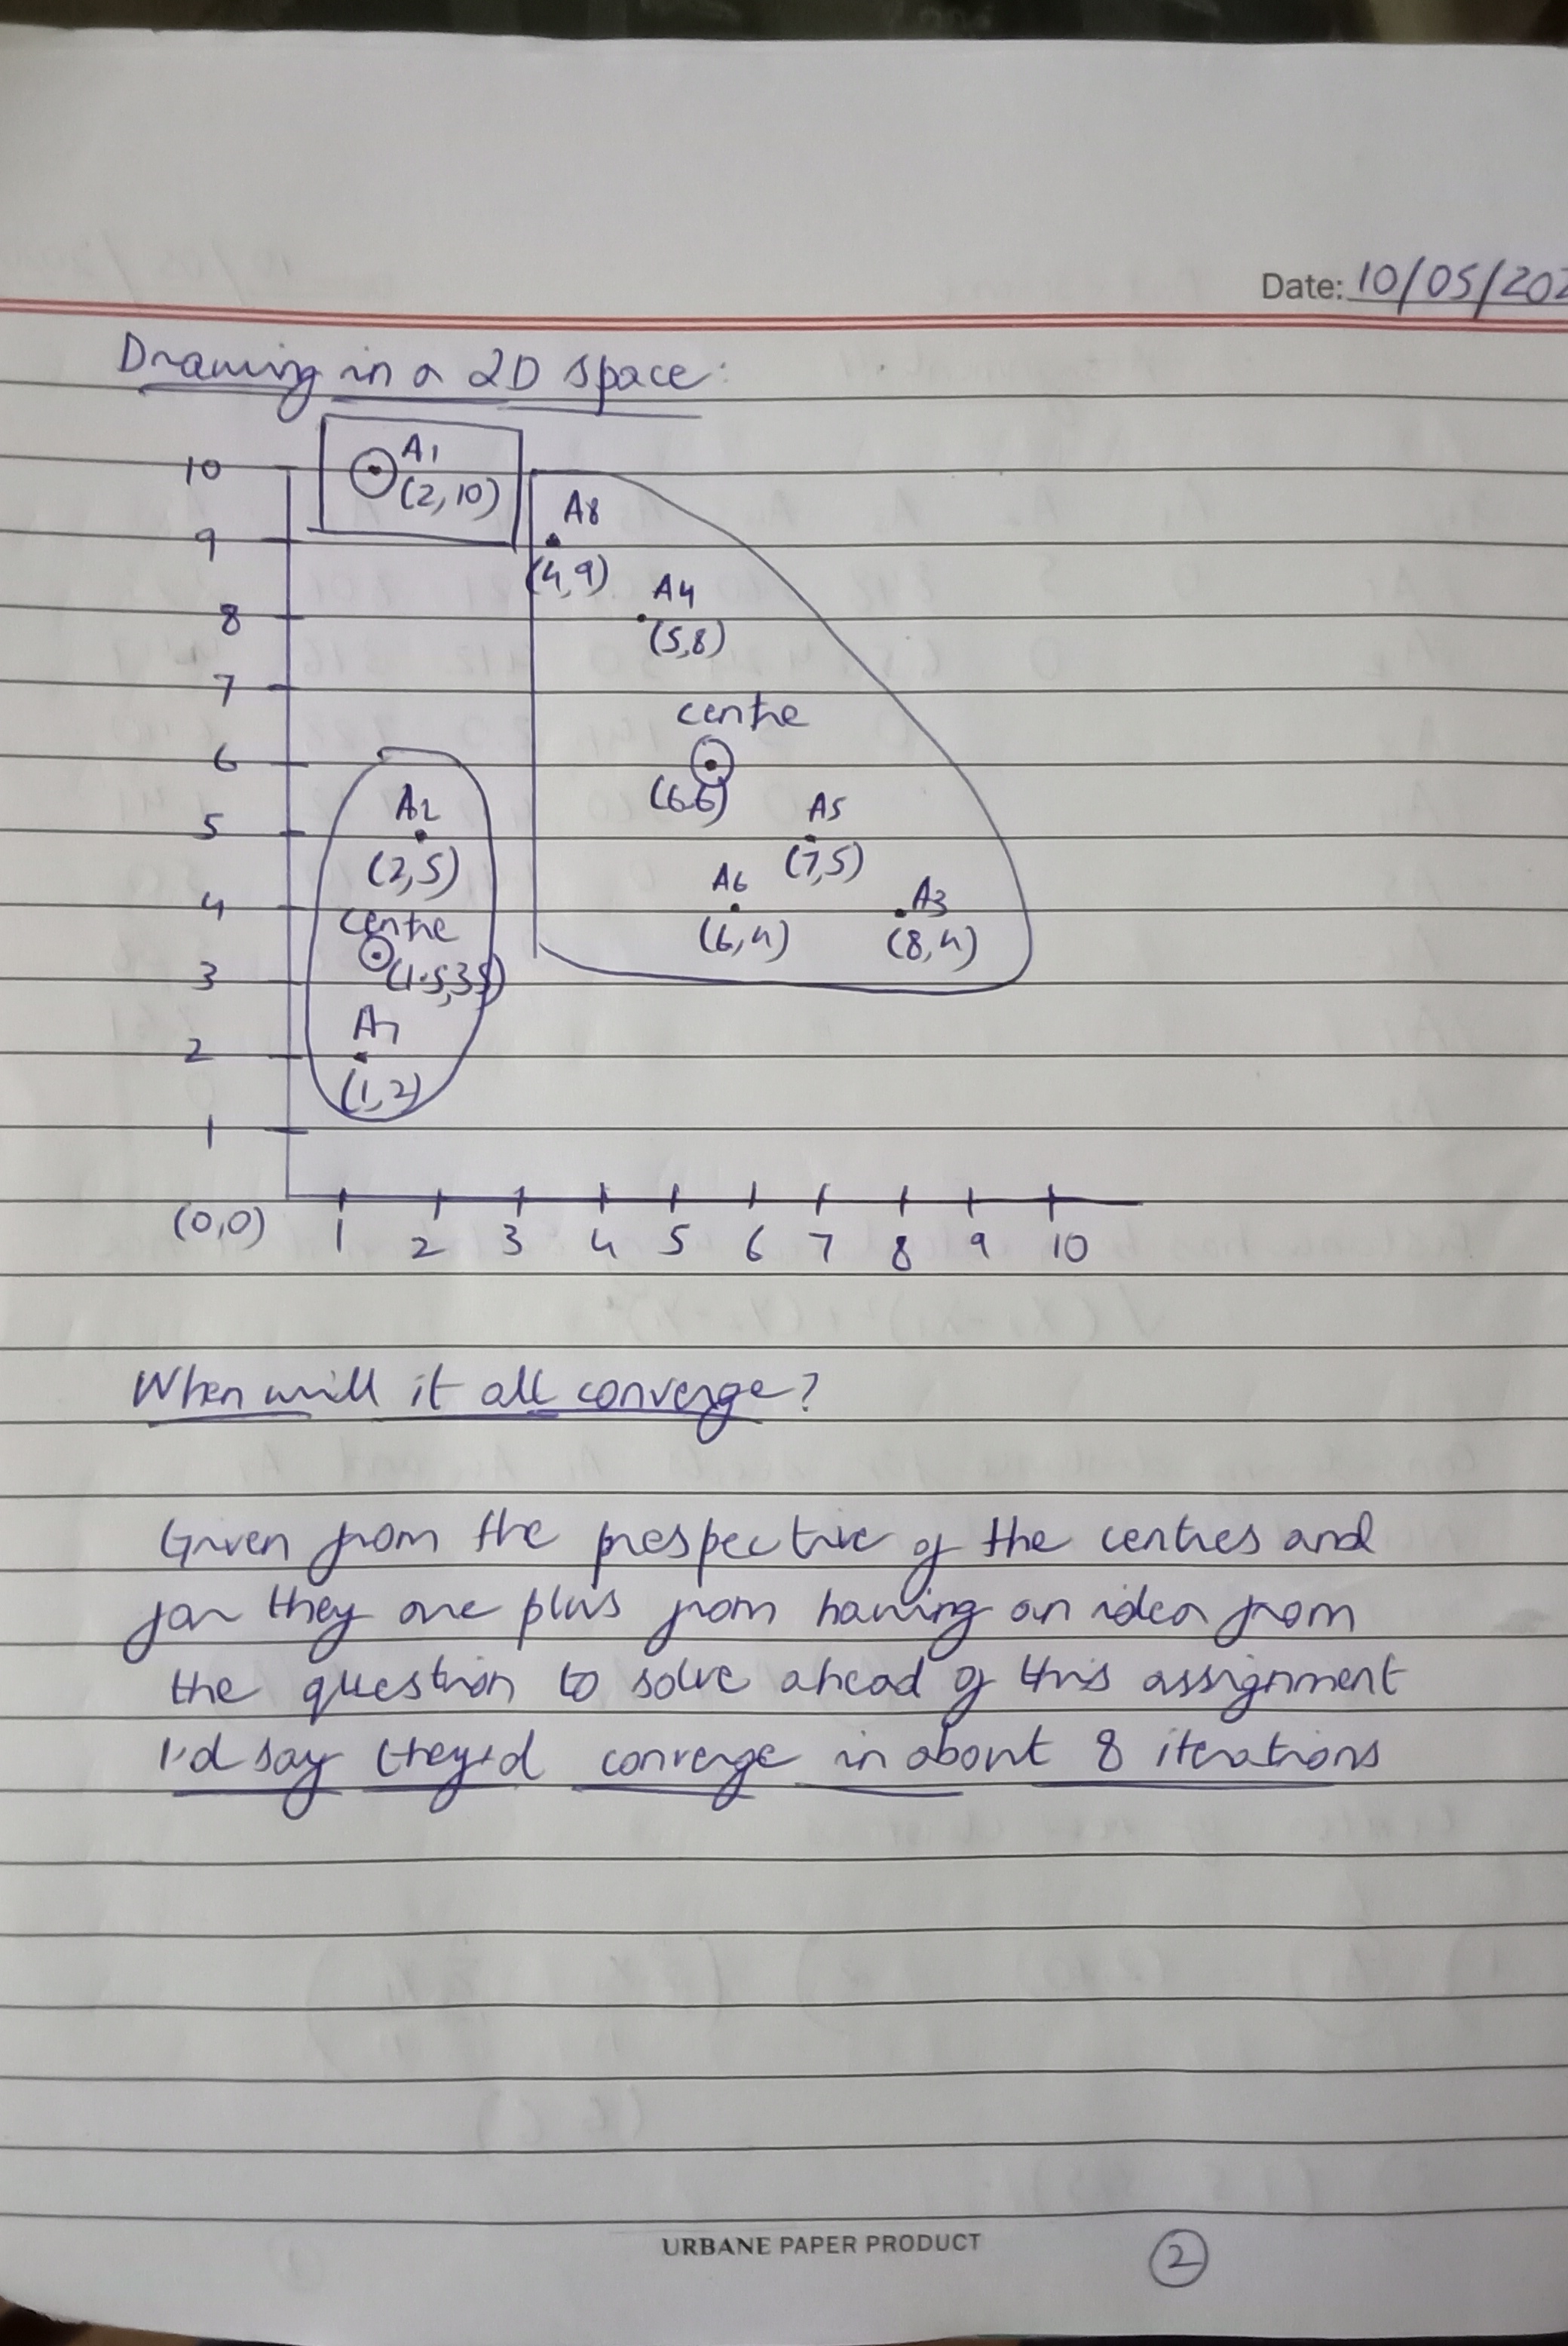
\includegraphics[width=\linewidth]{2.jpg}
  \caption{Drawn in 10x10 space}
  \label{pic2}
\end{figure}

\clearpage

\section{Hierarchical Clustering}

Using hierarchical clustering algorithms (Single, Complete, Group Average and Distance b/w centroids) and Euclidean distance to cluster the following 8 points into 3 clusters. Using A1 = (2,10), A2 = (2,5), A3 = (8,4), A4 = (5,8), A5 = (7,5), A6 = (6,4), A7 = (1,2) , A8 = (4,9).

\begin{figure}
  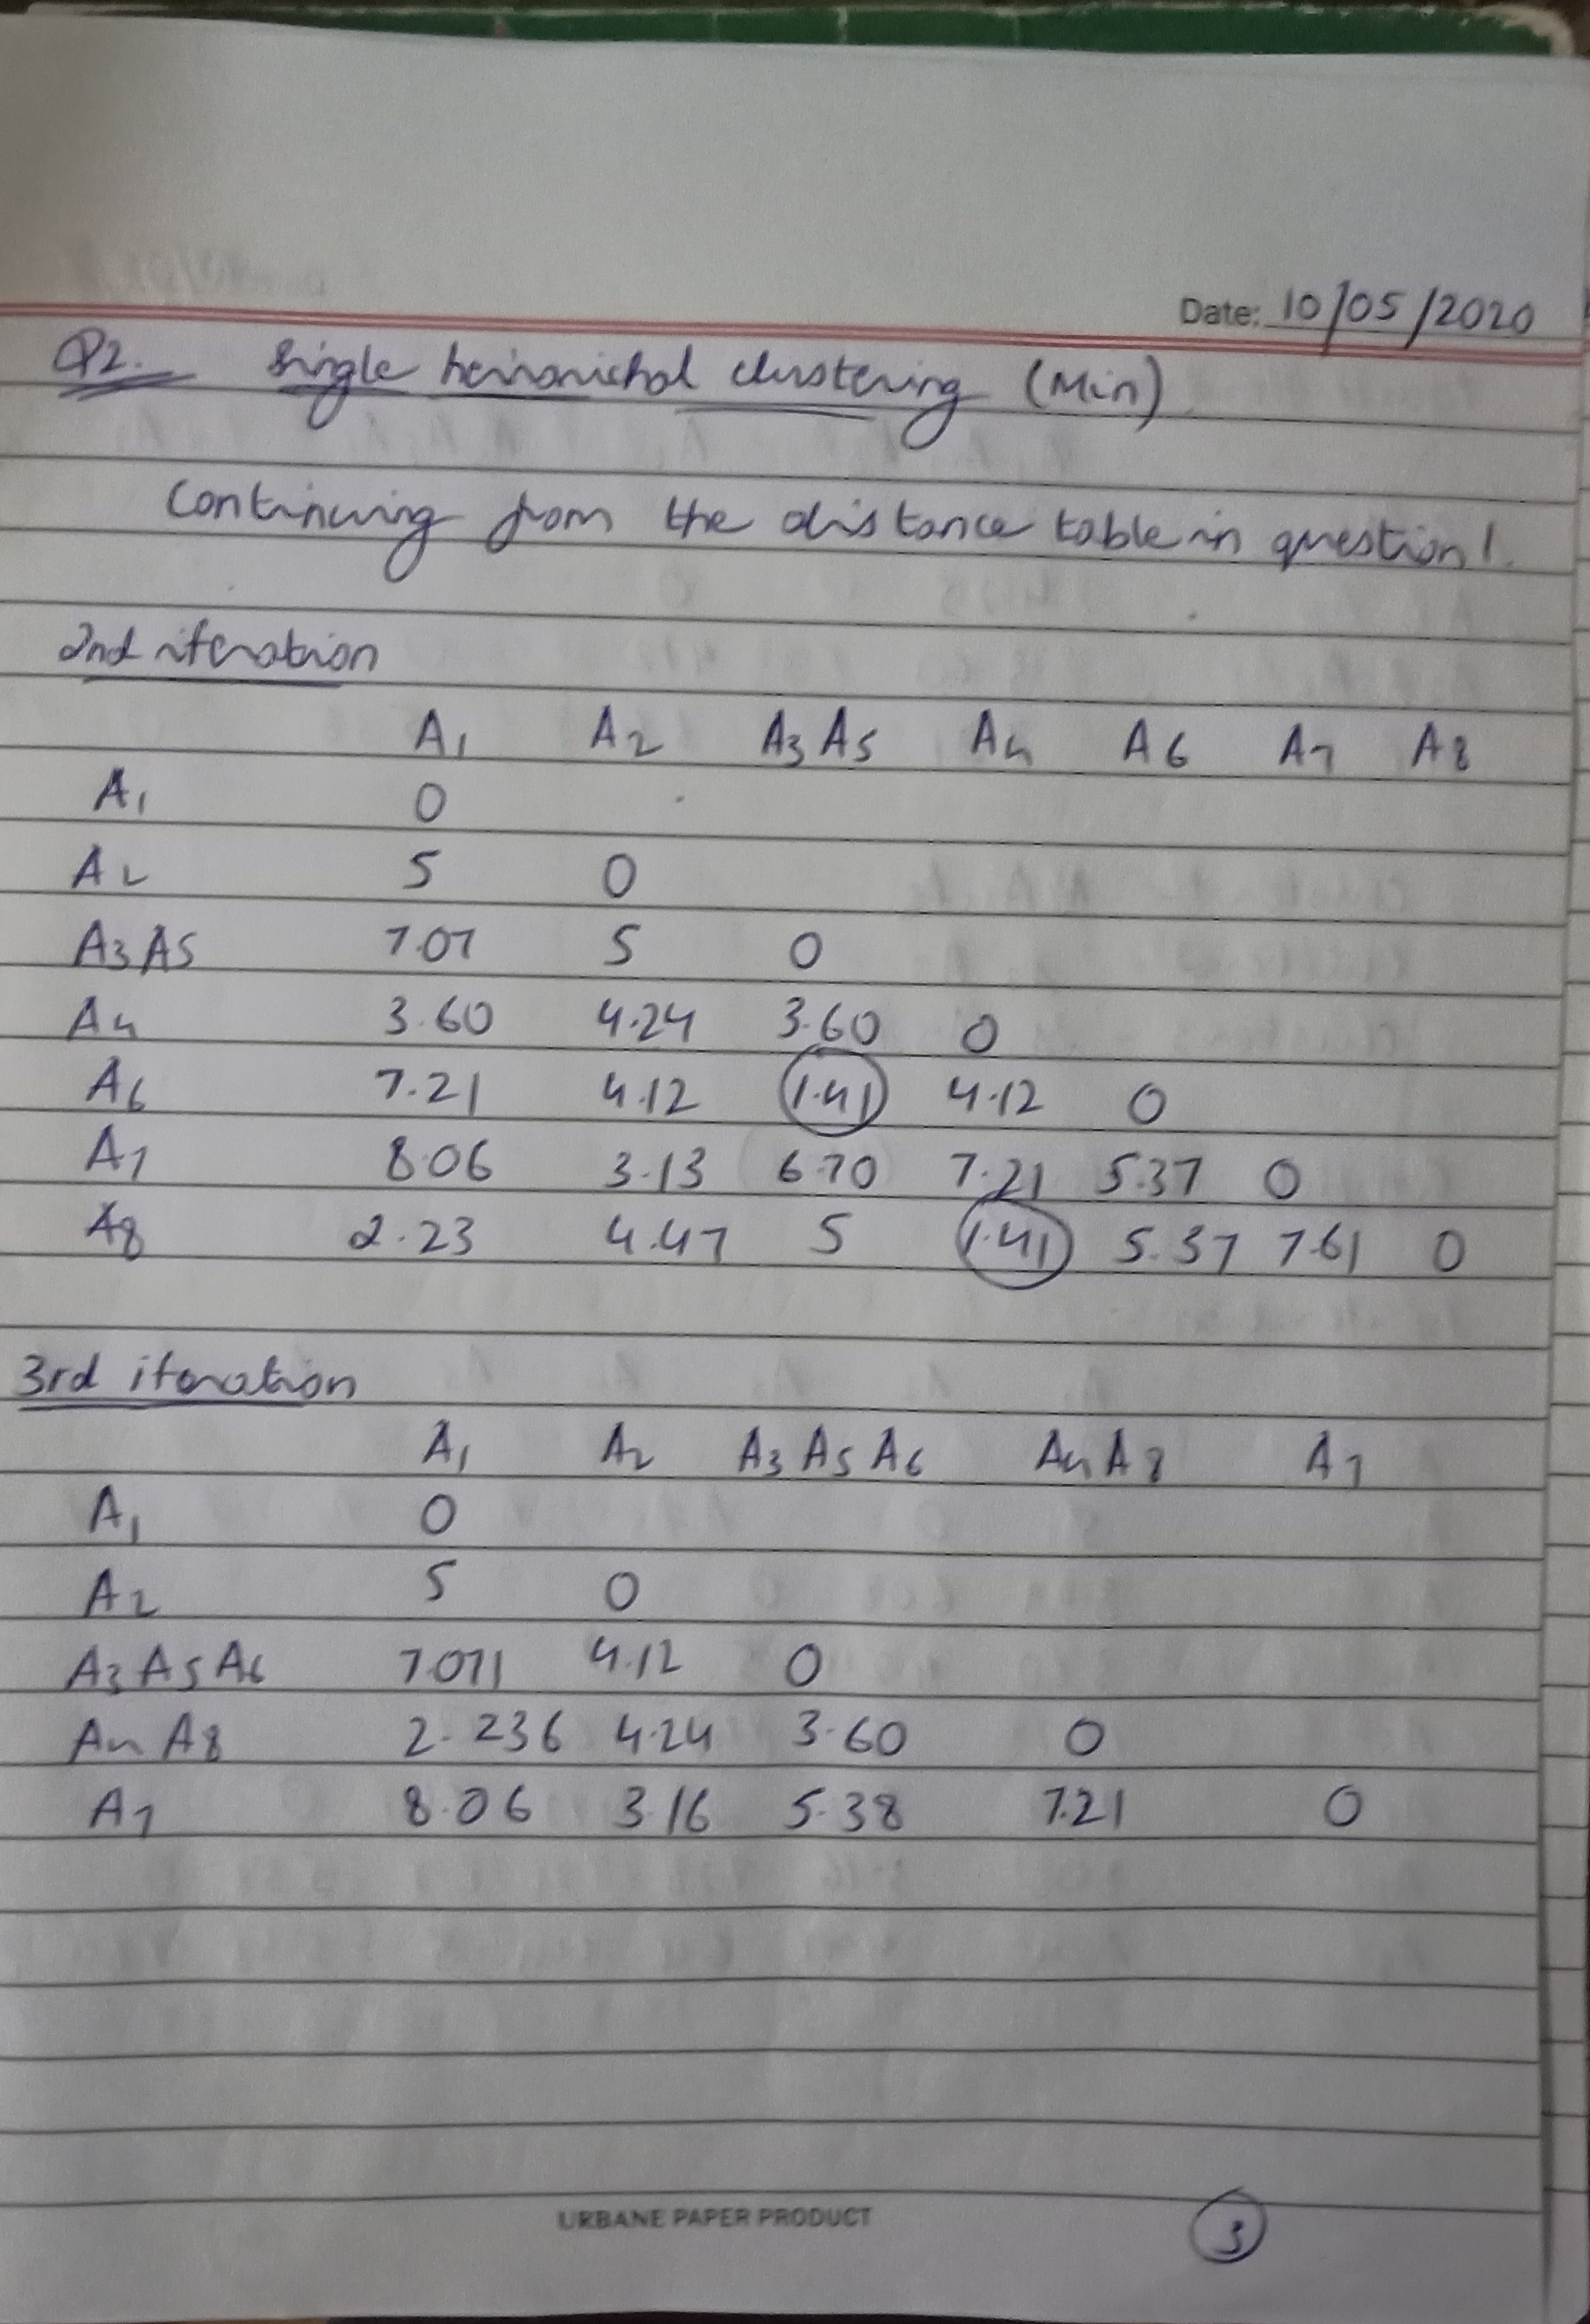
\includegraphics[width=\linewidth]{3.jpg}
  \caption{Single linkage}
  \label{pic3}
\end{figure}

\begin{figure}
  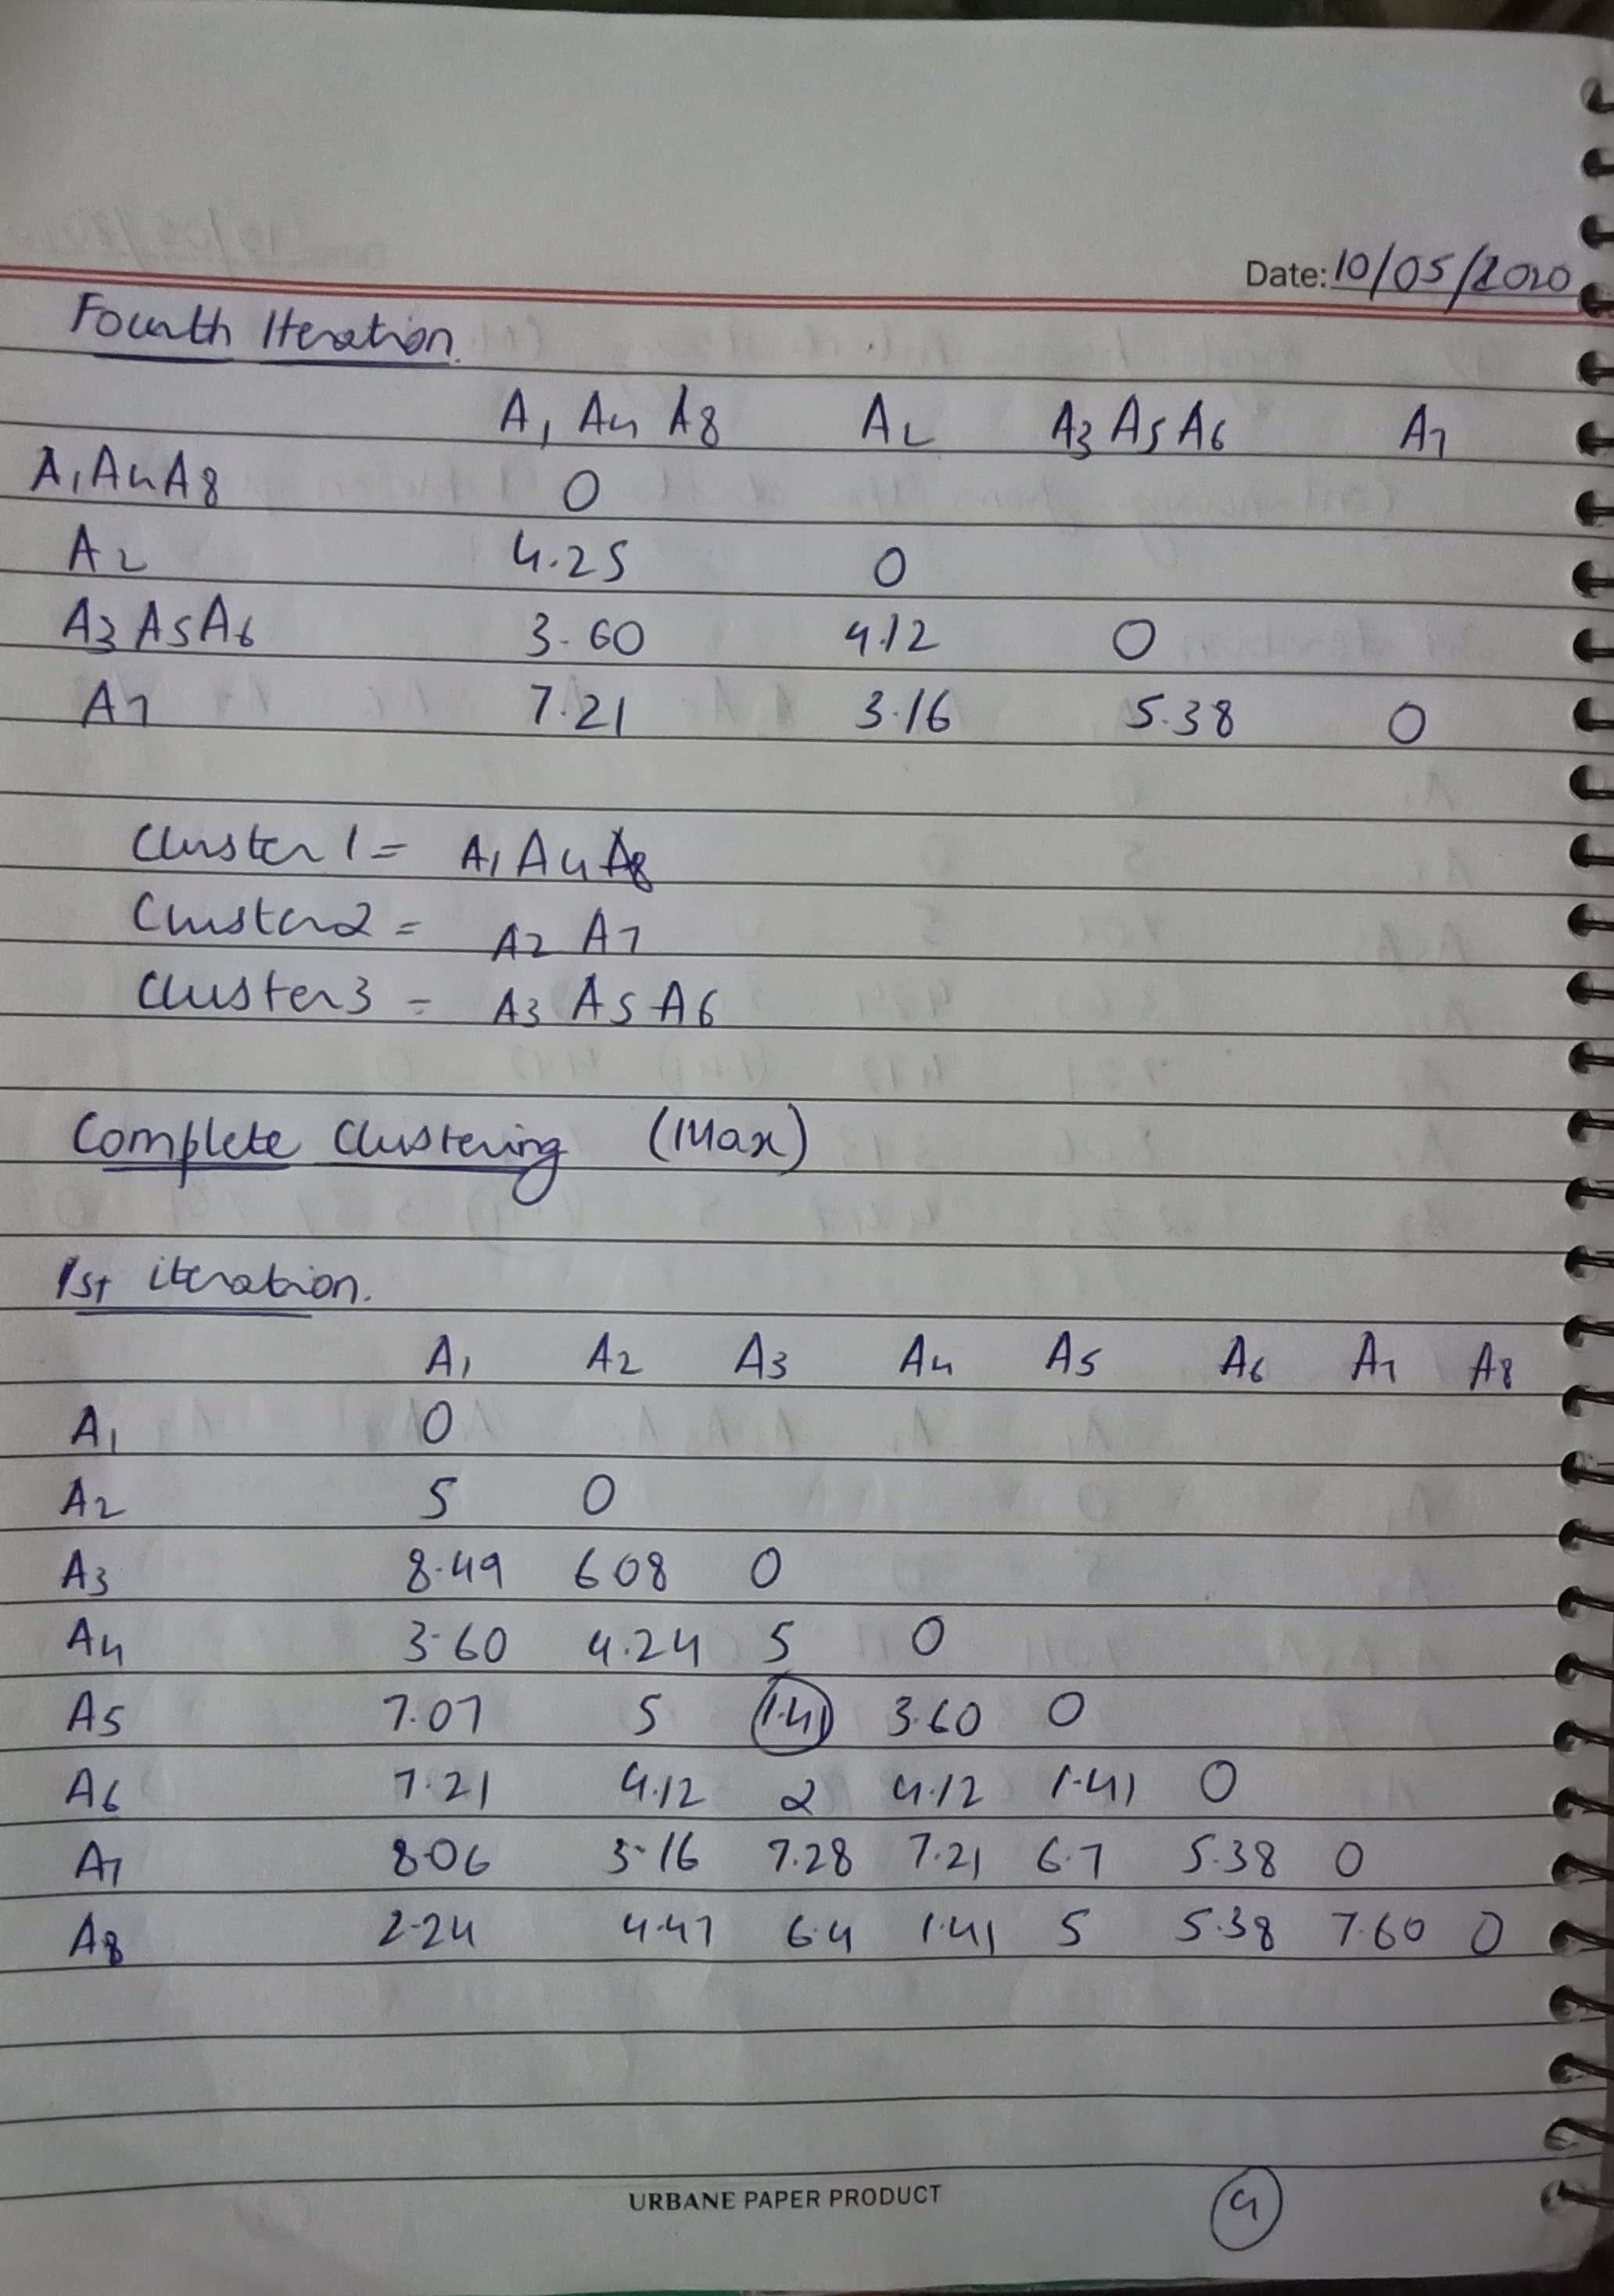
\includegraphics[width=\linewidth]{4.jpg}
  \caption{Complete linkage}
  \label{pic4}
\end{figure}

\begin{figure}
  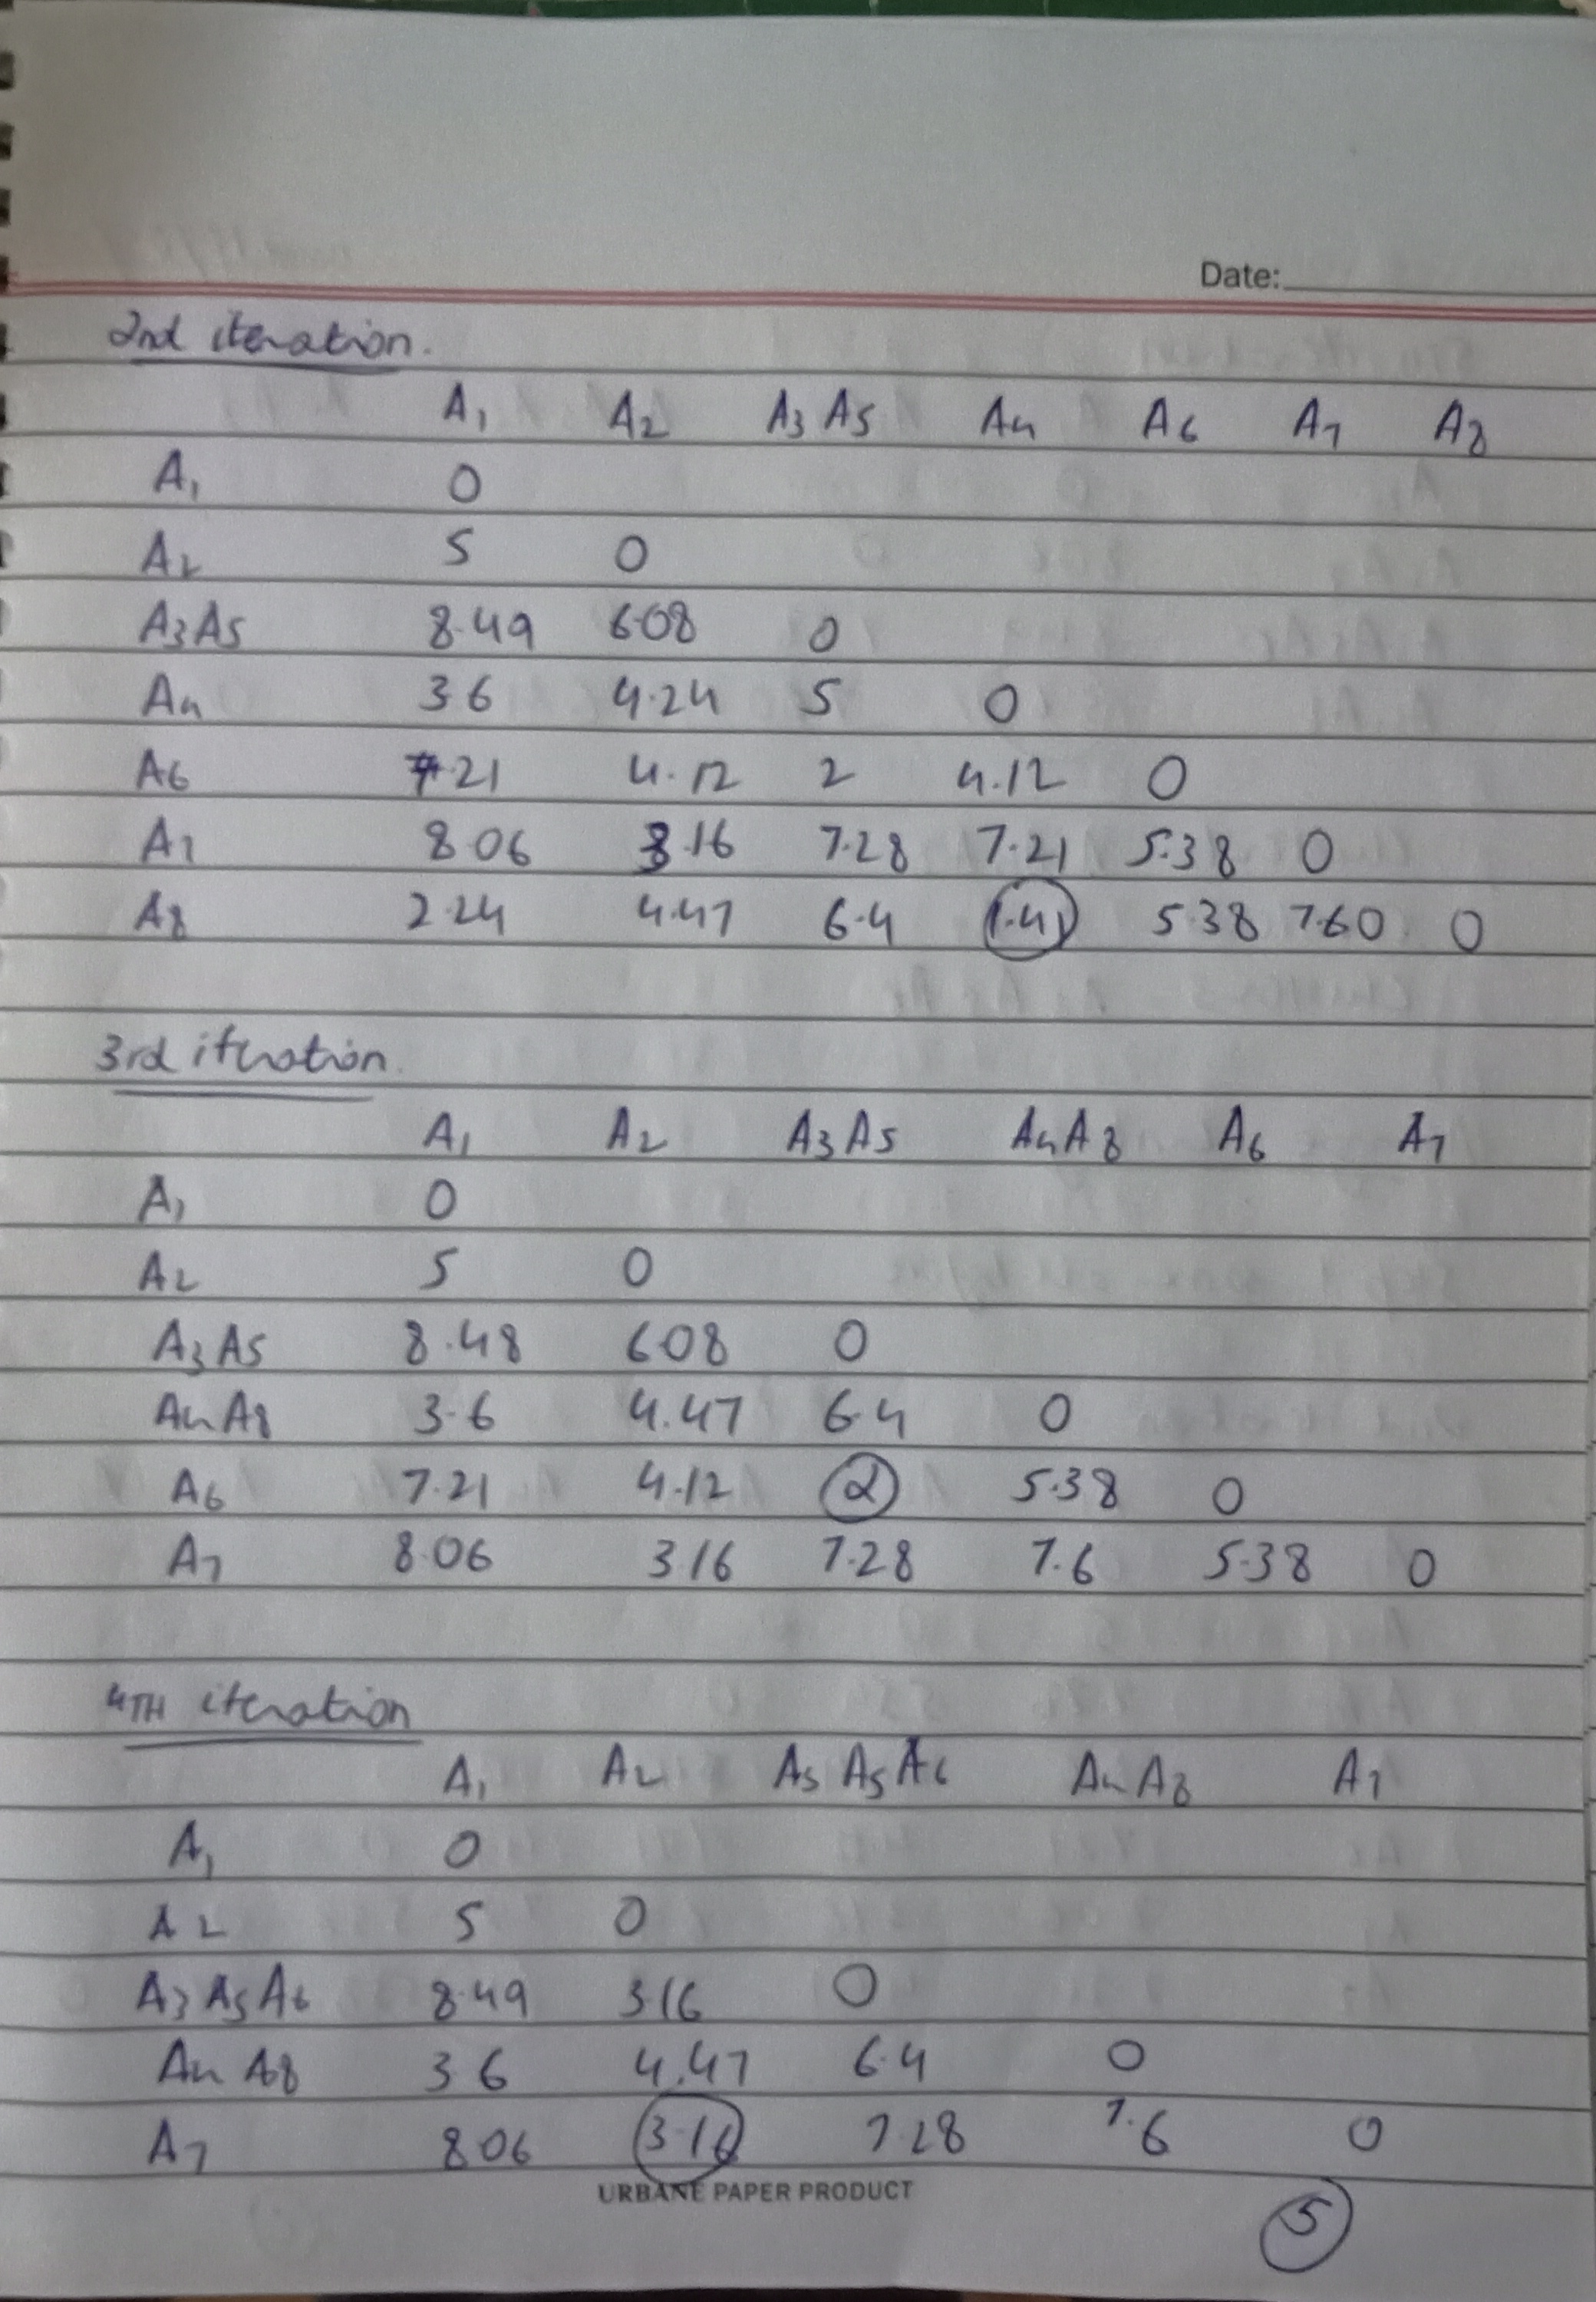
\includegraphics[width=\linewidth]{5.jpg}
  \caption{Complete linkage}
  \label{pic5}
\end{figure}

\begin{figure}
  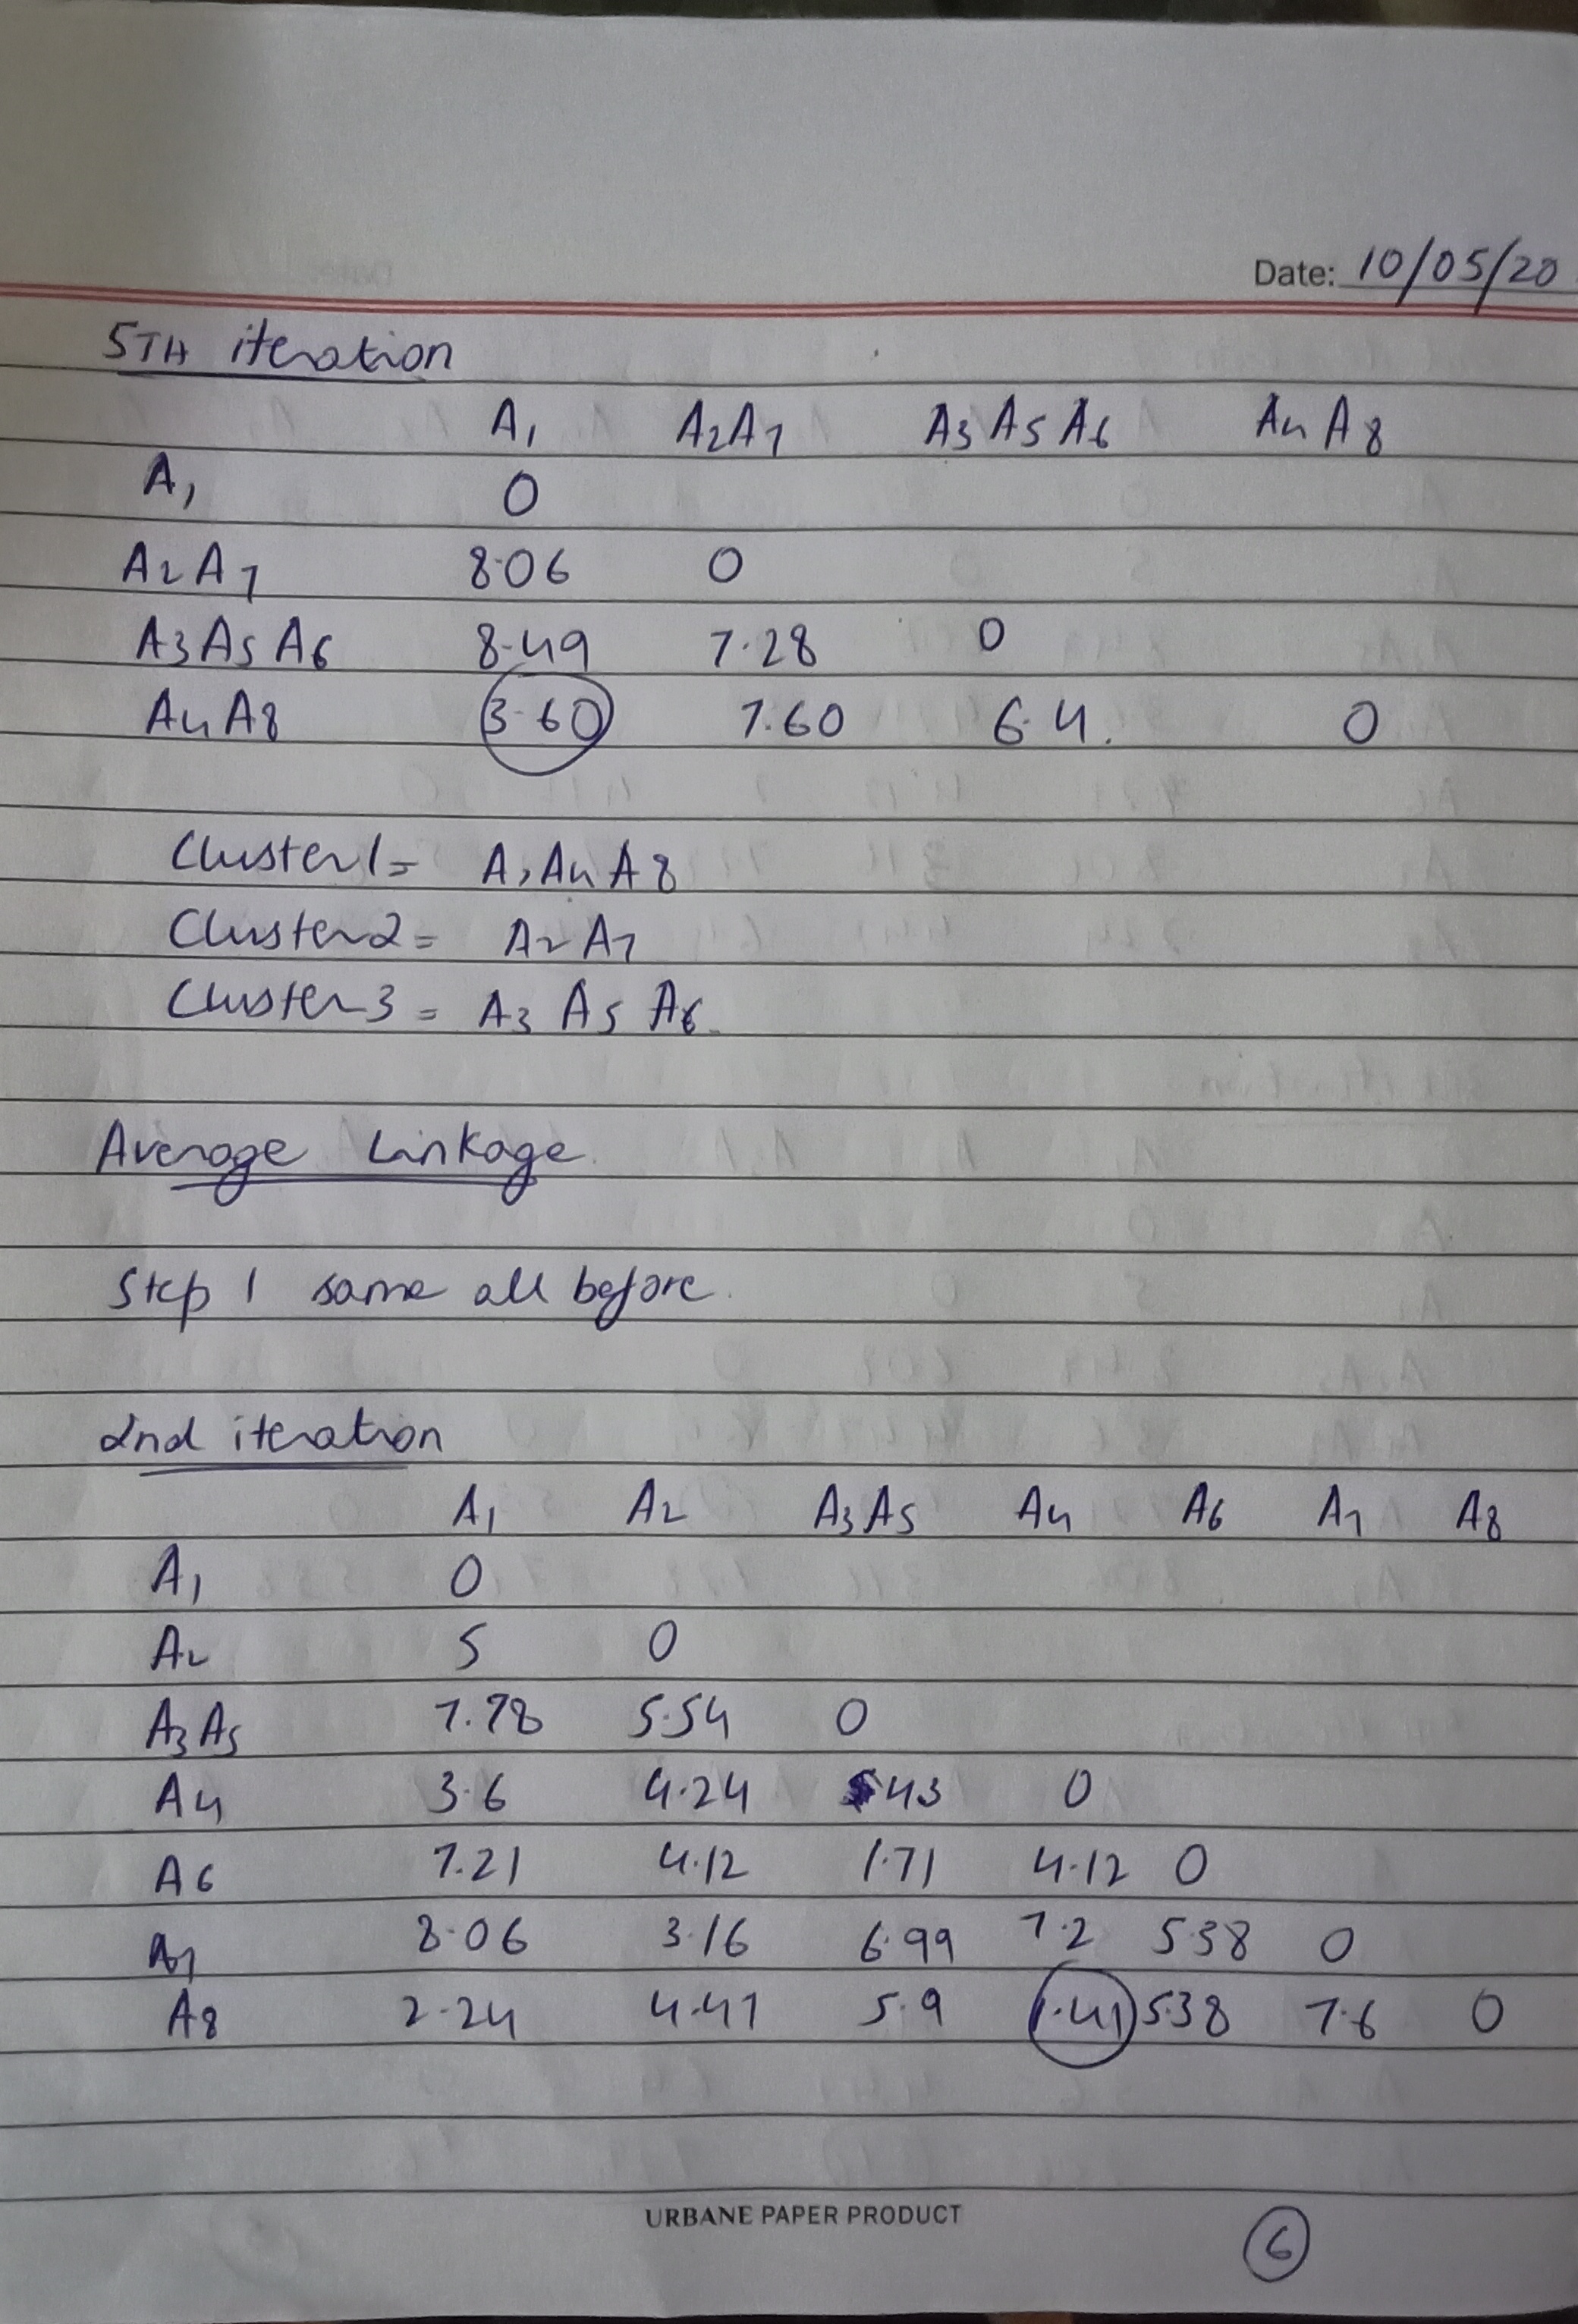
\includegraphics[width=\linewidth]{6.jpg}
  \caption{Average linkage}
  \label{pic6}
\end{figure}

\begin{figure}
  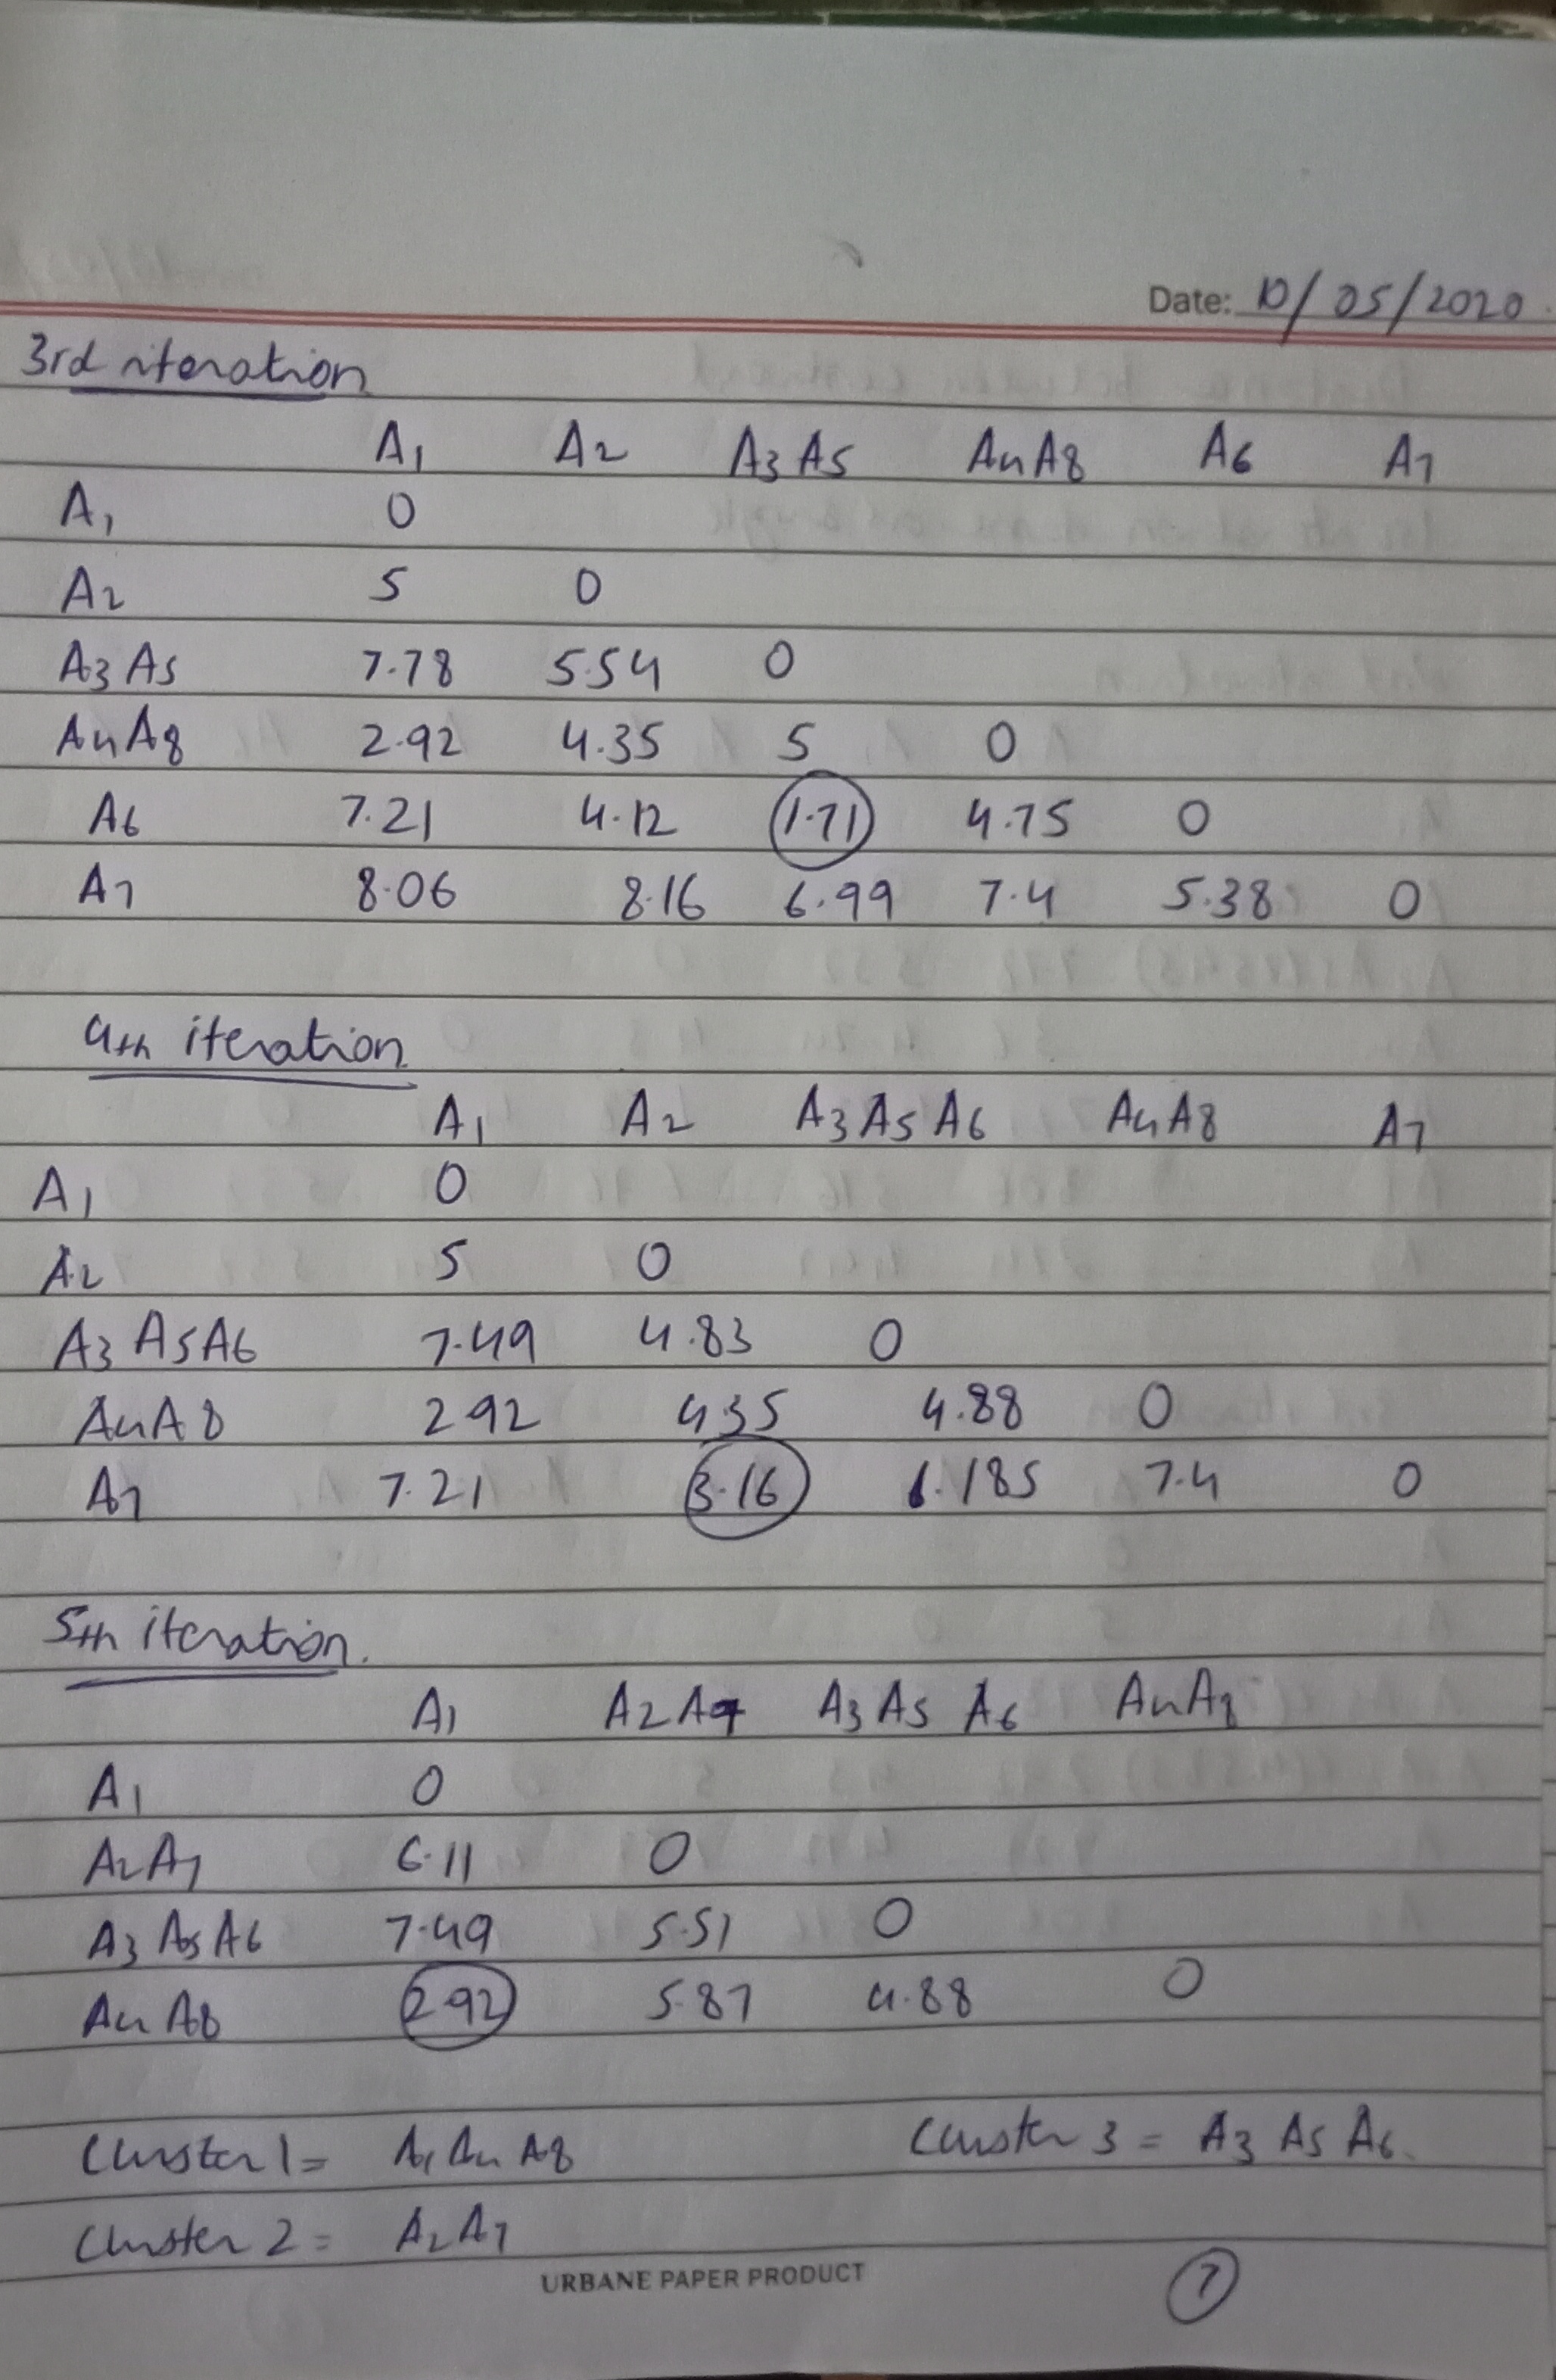
\includegraphics[width=\linewidth]{7.jpg}
  \caption{Average linkage}
  \label{pic7}
\end{figure}

\begin{figure}
  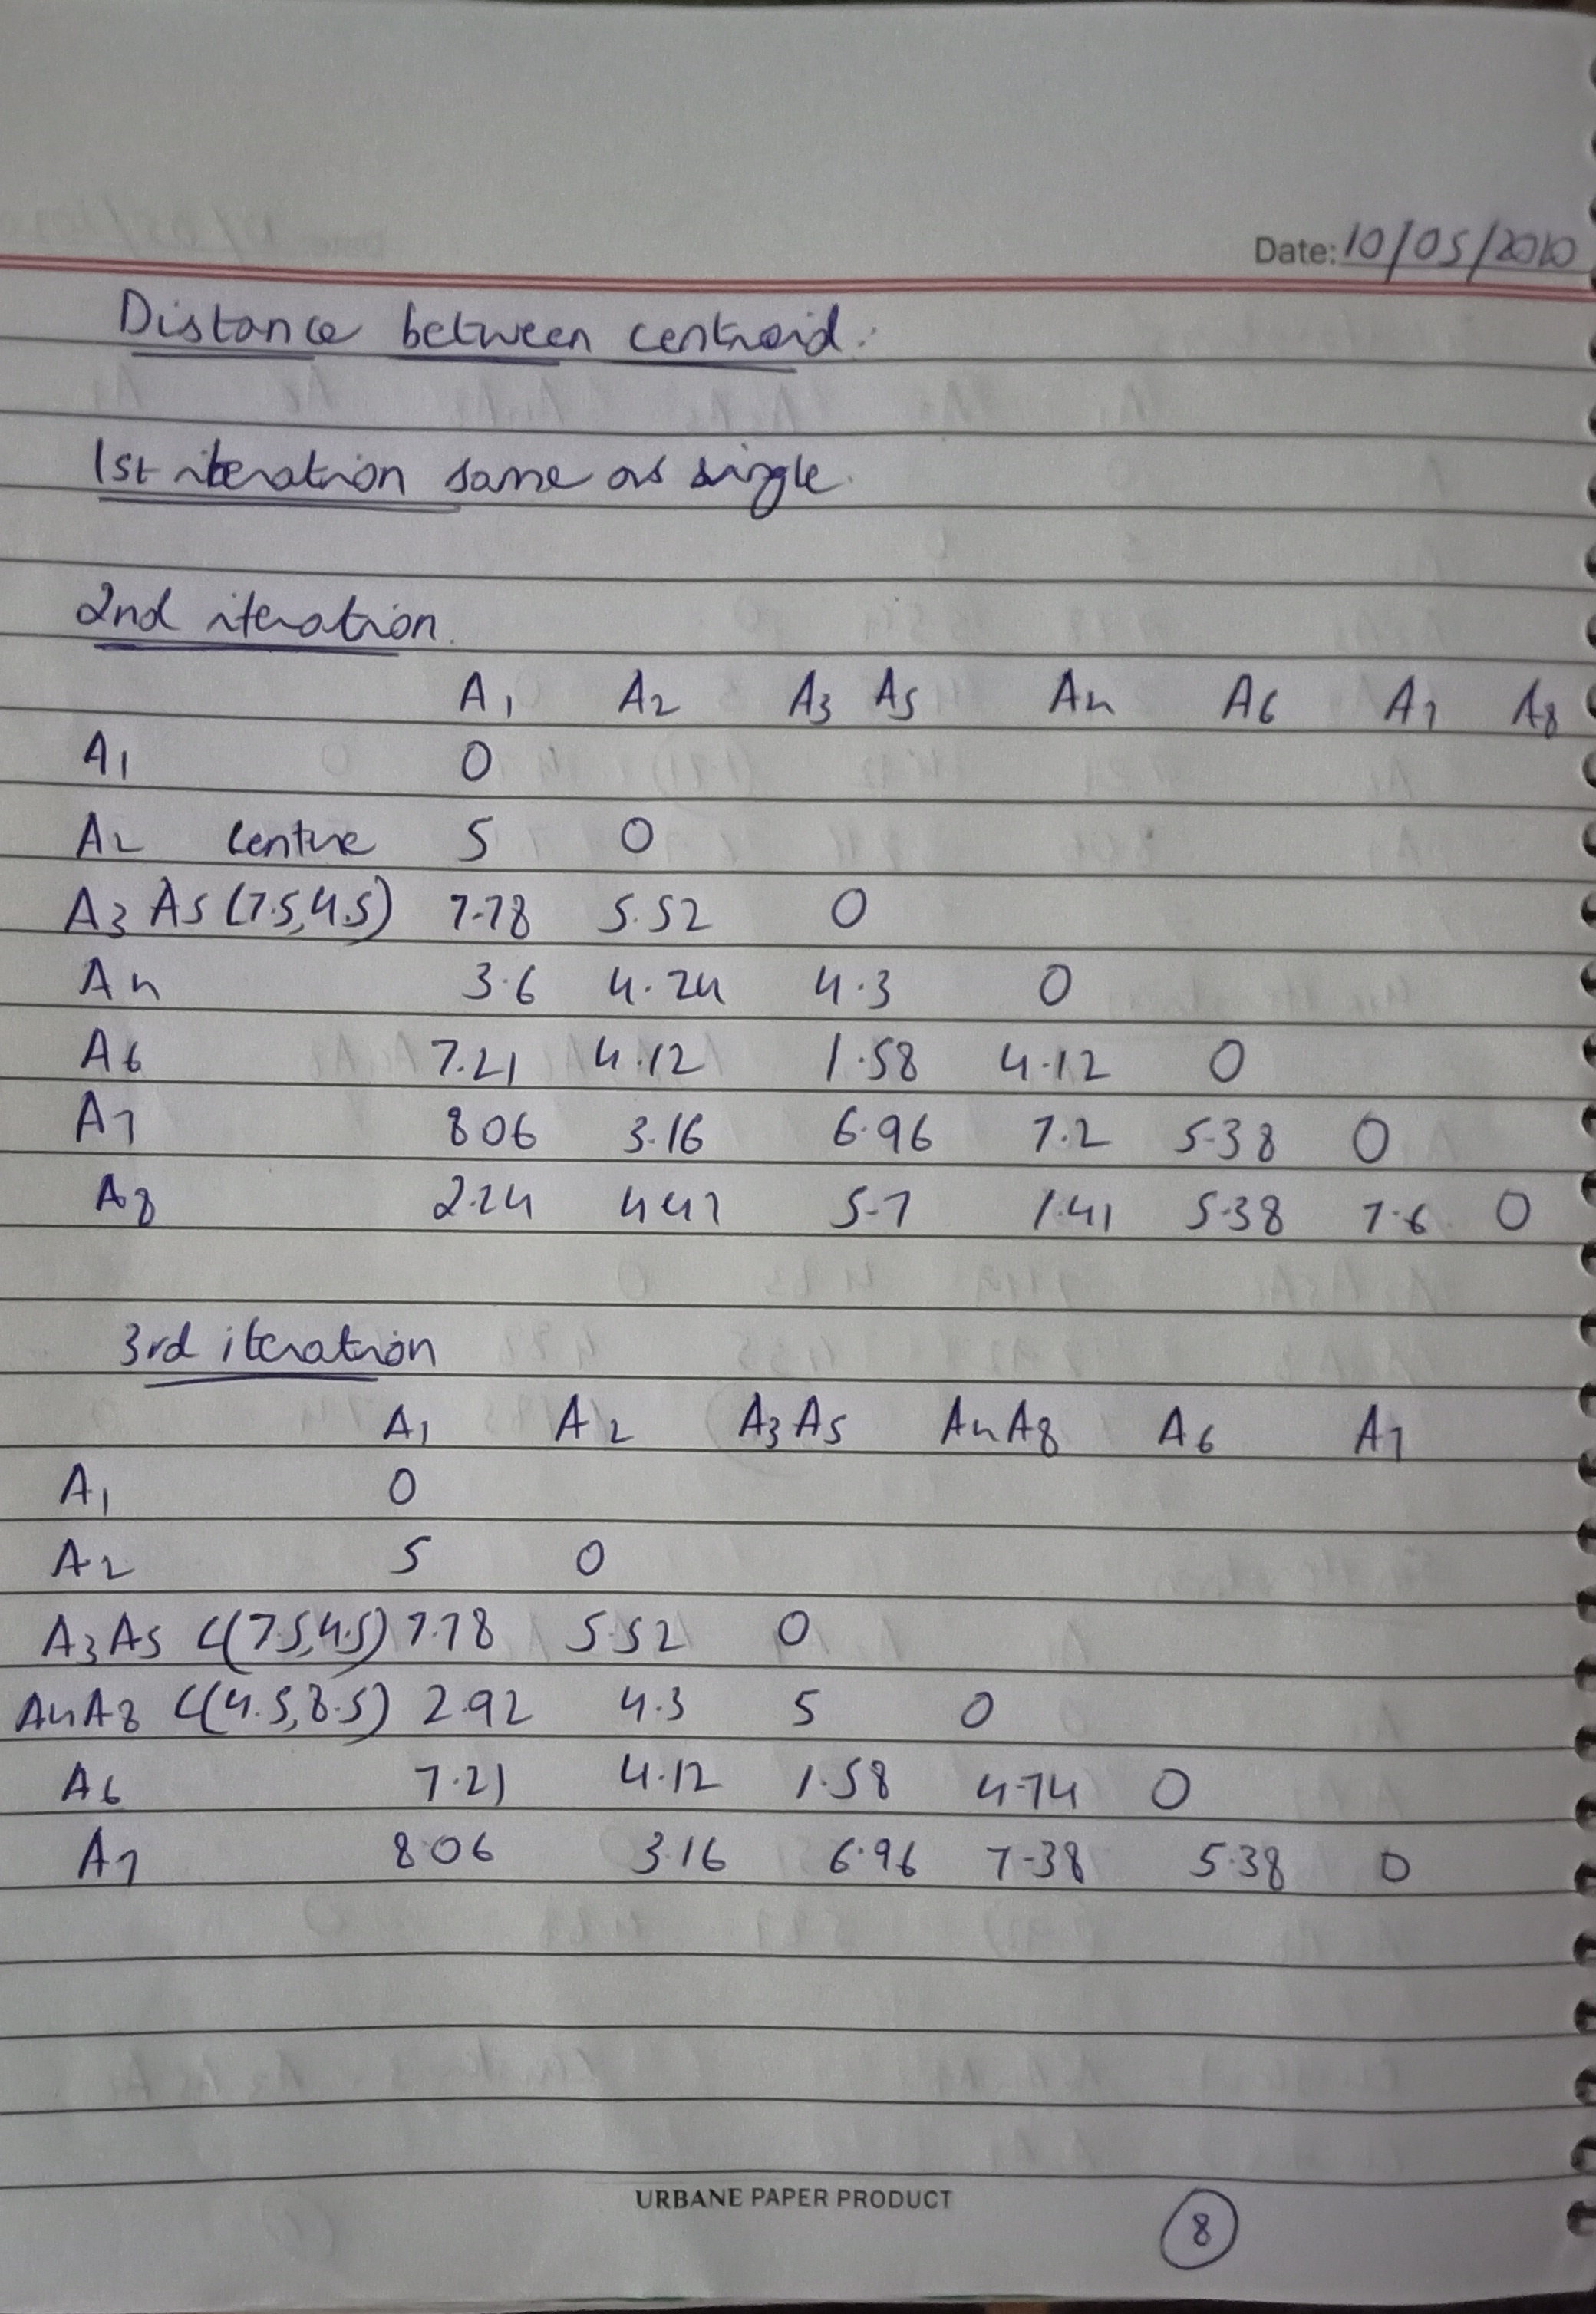
\includegraphics[width=\linewidth]{8.jpg}
  \caption{Distance between centroid}
  \label{pic8}
\end{figure}

\begin{figure}
  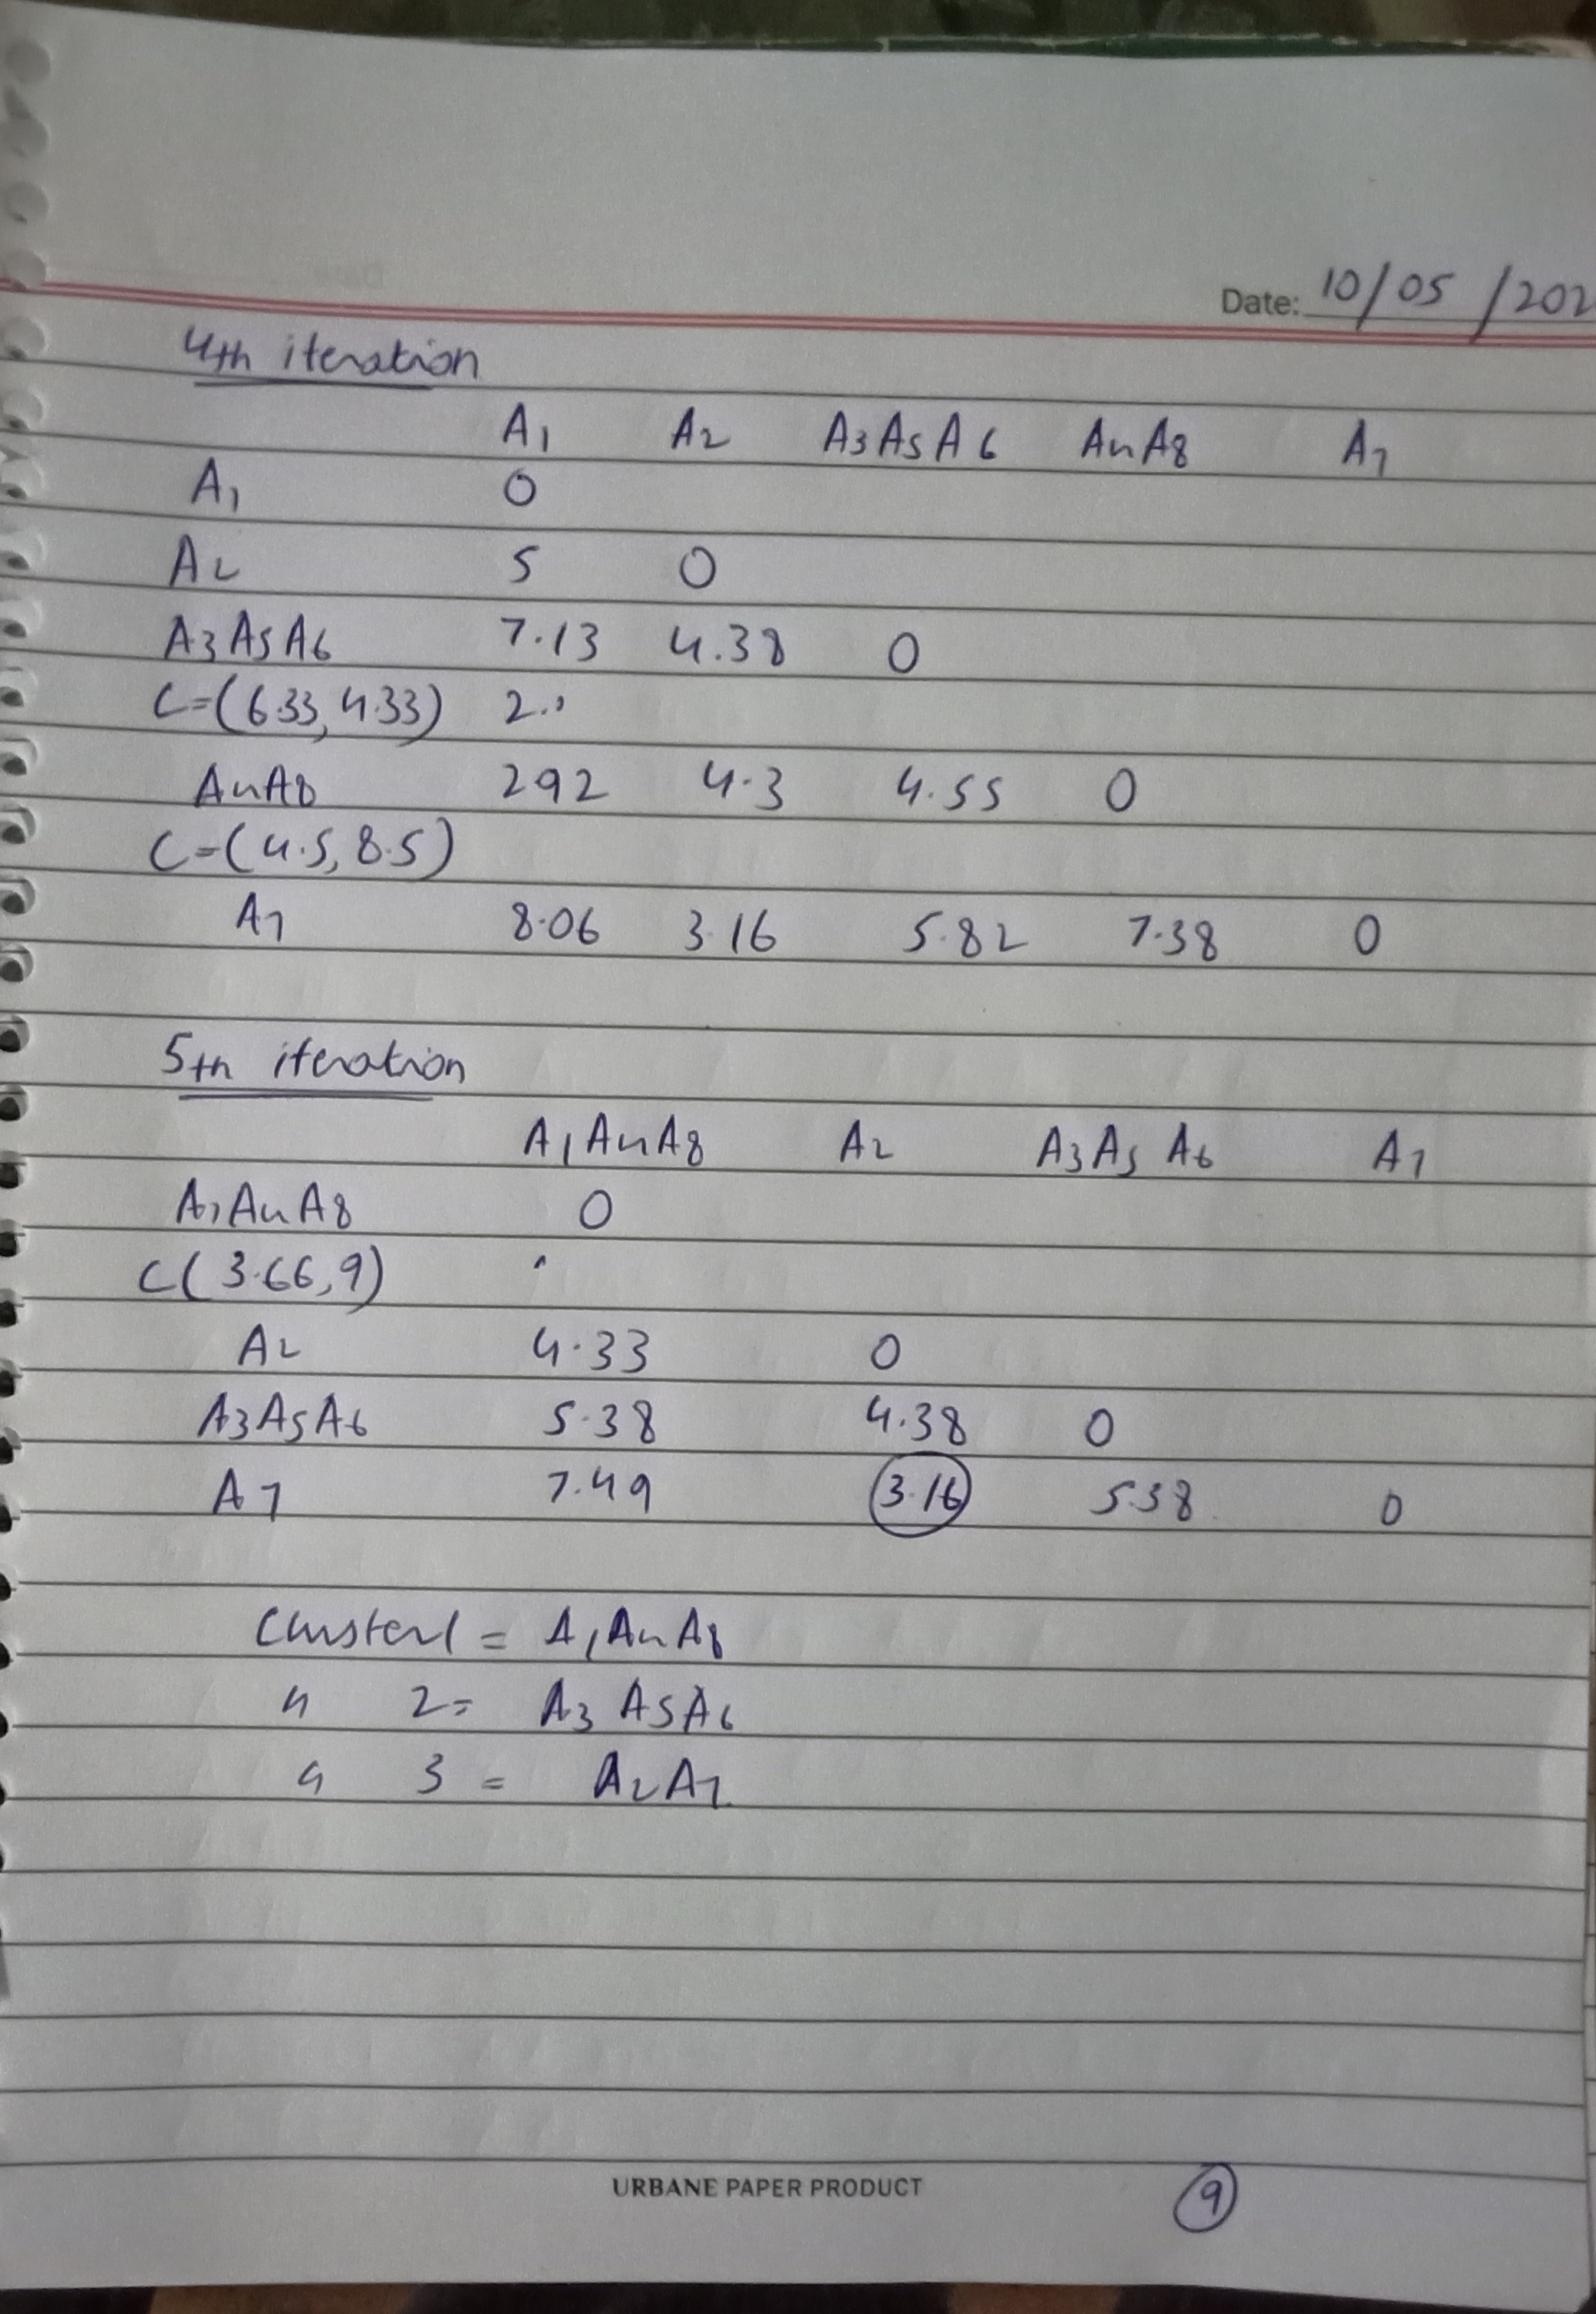
\includegraphics[width=\linewidth]{9.jpg}
  \caption{Distance between centroid}
  \label{pic9}
\end{figure}

\clearpage

\section{Paper Summary}

Review a paper of your choice on Soft Clustering e.g. Fuzzy Kmeans (One Page Summary). \newline

The following is a summary from the paper \textit{Fuzzy C- Means Algorithm- A review} by \textit{R.Suganya and R.Shanthi} it can be cited from the following link, \url{http://www.ijsrp.org/research-paper-1112/ijsrp-p1168.pdf}.
The paper describes in an informative way how there are 2 kinds of clustering, \textbf{Hard Clustering} the one which is usually opted for where each and every points is clustered in to a single group. On the other hand is \textbf{Soft Clustering} where every single point can be selected in to multiple groups or clusters depending on the criteria and means of clustering or feature selection. \textit{Fuzzy C Means} or FCM for short is a part of classical fuzzy clustering algorithms and this paper discusses it in detail and explains all the mathematical happenings of this algorithm. It is the most commonly used hard clustering algorithms present it was developed by \textit{Joe Dunn} in 1974 for a special case of $ K=2 $. Instead of classifying a point to a single special cluster, the objects on the boundaries between several classes are not forced to fully belong to one of the classes, but rather are assigned membership degrees between 0 and 1 indicating their partial membership.
Some Pros and cons by the paper are:
\begin{enumerate}
	\item Advantages
	\begin{enumerate}
		\item Unsupervised
		\item Converges
	\end{enumerate}
	\item Limitations
	\begin{enumerate}
		\item Long computational time
		\item Sensitivity to the initial guess (speed,local minima)
		\item Sensitivity to noise (outliers, NaN values)
	\end{enumerate}
\end{enumerate}

To overcome the difficulties presented by FCM another variant of the algorithm \textit{Probabilistic C Means} was presented which by the name proves that it works on the probabilities of distant points and keeps calculating clusters until each and every point has at least one cluster to represent with the probability of them being the part of that cluster a minimum of 0.5.It improves on the previous approach by being able to cluster noisy data more accurately and efficiently whereas the disadvantage of being sensitive to initialization is still present. This model was further perfected by means of \textit{Fuzzy Probabilistic C Means Algorithm} aka FPCM. It utilizes both, the typicality or feature extractions of fuzzy means plus the probability model of the possibilistic model. It ignores the noisy sensitivity deficiency of FCM.

\end{document}
